\documentclass[11pt, a4paper]{article}
%\usepackage[danish]{babel}
\usepackage{amsmath}
\usepackage[utf8]{inputenc}
%\usepackage{xfrac}
\usepackage{amsfonts}
\usepackage{amssymb}
\usepackage{tikz}
\usepackage{array}
\usepackage{cancel}
\usepackage{ulem}
\usepackage{graphicx}
\usepackage[a4paper]{geometry}
\usepackage{gauss}
%\usepackage{mathtools}
\usepackage{amsmath}
\usepackage{lastpage}
\usepackage{fancyhdr}
\usepackage{multirow}
\usepackage{listings}
\setlength{\headheight}{15.2pt}
\pagestyle{fancy}
\fancyhf{}
\lhead{Mads Anthony, MANA} %husk denne
\rhead{Side\ \thepage\ af\ \pageref{LastPage}} %husk 2 builds for dette!
%\usepackage[ansinew]{inputenc} 
\usepackage{enumerate}
%dot2tex loads
\usetikzlibrary{shapes}
\begin{document}
\author{Mads Anthony}
\section{Background}
This section will work as the background section for things related to neural oscillations. One of the main motivation to incorporate frequencies into evolutionary methods, is that research indicates that neural oscillations could be beneficial to switching between multiple tasks. It therefore makes sense to have a section that summarise that particular research as well as a general description of neural oscillations.
\\
\\
However since this topic is a research field of it's own, this section will only give a general perspective of neural oscillations, as the main focus in this report will be in the computer science domain.
\subsection{Neural oscillation}
Neural oscillations was first observed in the human brain in 1924 by placing electrodes on the scalp of the head using a method called Electroencephalography (EEG) [Hans Berger]. EEG is able to record the electrical activity of the brain, by recording the spikes of the neural firings.
\subsection{Synchrony}
\subsection{Communication through coherence (CTC) hypothesis}
\subsection{Research Papers}
\subsubsection{Synchronous Oscillatory Neural Ensembles
for Rules in the Prefrontal Cortex}
The results of the following paper suggest that the task of switching between rules could be related to neural oscillations. They found evidence that there was an increase in synchrony at the beta frequencies for rule 1, and when they switched to rule 2 there was an increase in synchrony in the alpha frequency.
\\
\\
The research paper used two monkeys to switch between two rules. The monkeys was given visual cue cards that had a line placed in the center of the card. The line could then vary in color and could be aligned either vertical or horizontally. The monkeys should then look either left or right dependent on what rule was in effect. The two rules either made use of the color or the orientation of the line. So if the color rule was in effect, the monkey had to look left if the line was red and look right if it was blue. Similiar if the orientation rule was effect, the monkey had to look left if horizontal and right if vertical.
\\
\\
While the monkeys were performing the different tasks, local field potentials (LFP) was recorded from multiple electrodes at the prefrontal cortex (PFC).
\begin{figure}[!ht]
\centering
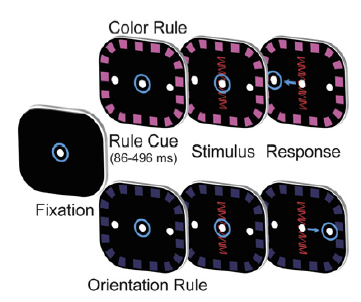
\includegraphics[scale=0.5]{MonkeyRules}
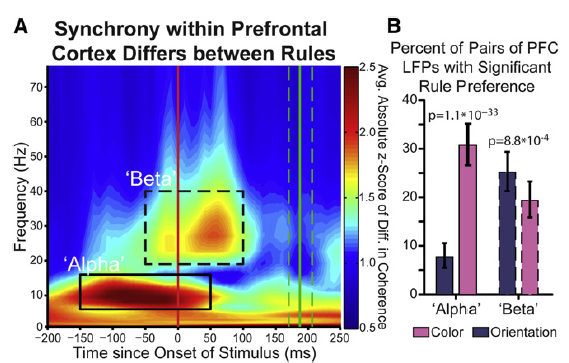
\includegraphics[scale=0.5]{MonkeyResults}
\caption{}
\end{figure}
\\
As can be seen in figure (x), there is a clear increase in synchrony in the alpha "band" when the color rule is in effect and a significant increase in the bata "band" when the orientation rule is in effect.
\end{document}